\section{Incremental Cycle Analysis}

Our intention is to support a design and analysis work flow that includes 
incremental analysis steps.  For example, a designer may analyze part of the design before integrating it into a larger part of the system.  In our work flow, we envision storing the results of that first analysis along with some interface data to reduce the cost of the second analysis.  The same should hold true for the system design.  We should be able to analyze the system design efficiently, calculating incremental analysis interfaces.  When the system models are revised, whether by adding, removing, or modifying components we can isolate the effects of the change on the cost of the analysis.  Cycle analysis is a useful example, but our aim is to tackle this problem more generally.

\subsection*{Formal Model}
\addcontentsline{toc}{subsection}{Formal Model}

Let $\mathbb{G}$ be a well-formed hierarchical graph (as in Bruni
\cite{graphs:hier_algebra}).  To get more comfortable with the notation,
first note that graph $\mathbb{G}$ itself (without hierarchical structure)
can be given as:

\begin{equation}
\mathbb{G} = (\parallel x) \parallel (\parallel_{(u,v) \in \mathcal{E}} l < u, v >)
\end{equation}

which is the parallel composition of the graphs induced by individual edges of $\mathbb{G}$, merged at their common vertices.

Let $C(\mathbb{G})$ be the set of elementary cycles in $\mathbb{G}$, and 
let $P(\mathbb{G}, u, v)$ be the subgraph of $\mathbb{G}$ containing all of
the paths from vertex $u$ to vertex $v$.

Consider a design of type $W$.  Let $W_{\bar{x}}^p [G]$ 
represent a parent design object in a graph hierarchy with interface
vertices $\bar{x}$, 
and let $W_{\bar{x}_i}^{c_i} [G]$ be the children
of $W^p$ 
($\llbracket W^{c_i} \rrbracket \subset \llbracket W^p \rrbracket$).  
Then neglecting vertex hiding and renaming 
to simplify the illustration, we have the following:

\begin{equation}
W_{\bar{x}}^p [\mathbb{G}] = W_{\bar{x}}^p [ (\parallel_{h} x_h) \parallel
(\parallel_{(j,k)} l< j,k >) \parallel (\parallel_{i} W_{\bar{x}_i}^{c_i} 
[\mathbb{G}]) ]
\label{eq:composition}
\end{equation}

Eq. \ref{eq:composition} describes the design $W^p$ in terms of its design 
children $W^{c_i}$, internal vertices $x_h$, and edges $l <j,k>$.   Fig. \ref{fig:hier_cycle} gives a simple example of a hierarchical graph with one child component and one cycle including vertices and edges within the child component.

\begin{figure}[htb]	
    \begin{center}
    \centerline{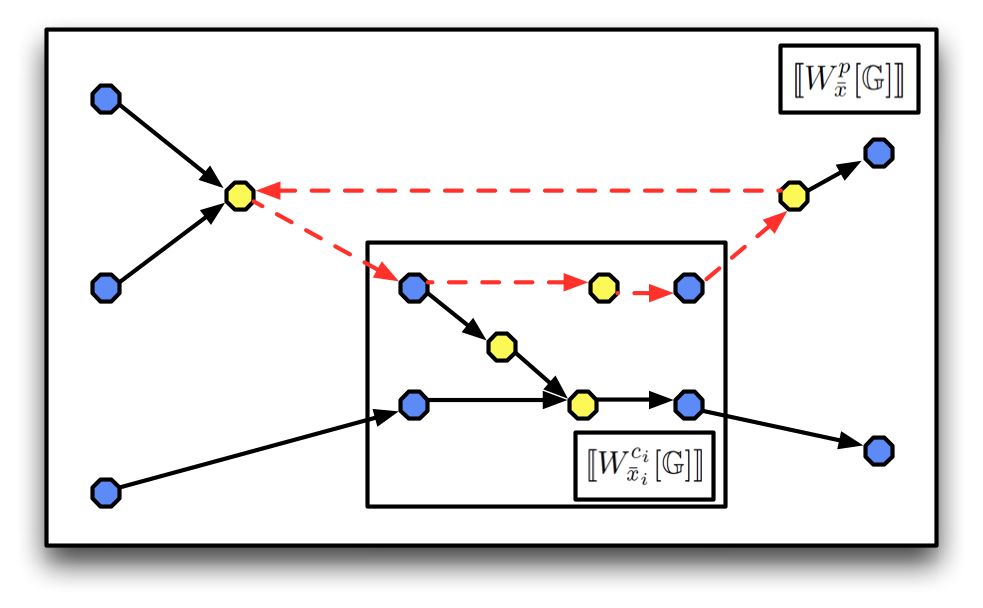
\includegraphics[width=0.7\columnwidth]{figures/original_graph.png}}
    \caption{Generic hierarchical graph model}
    \label{fig:hier_cycle}
    \end{center}	
\end{figure}

We introduce a new label $l_c$ into the sort for edges ($\mathcal{E}$),  
which is used to connect vertices at the boundaries of a design, 
abstracting the interface connectivity of the design. Introduce 
a new mapping $A: \mathcal{D} \rightarrow \mathcal{D}'$ from the 
designs of $\mathbb{G}$ to designs in a new graph $\mathbb{G}'$.  
$\mathbb{G}'$ is identical to $\mathbb{G}$, but adds the new edge
label.  This is the interface that we will use for incremental cycle
analysis.

\begin{align}
A( W_{\bar{x}_i}^{c_i} [\mathbb{G}] ) = & W_{\bar{x}_i}^{c_i} 
[ (\parallel_h x_h) \parallel 
(\parallel_{(j,k) \in \lfloor \bar{x}_i \rfloor \wedge P(\mathbb{G},j,k) 
\neq \emptyset} l_c <j,k>) \\
 & \parallel (\parallel_{(j,k)} l<j,k> )
\parallel (\parallel_m W_{\bar{x}_m}^{c_m} [\mathbb{G}]) ]) ] \nonumber
\end{align}

In this abstraction function the child designs are replaced by a much simpler
connectivity graph.  We introduce two functions to support the algorithm:

\begin{align}
&R(A(W_{\bar{x}}^{c_i} [\mathbb{G}])) = W_{\bar{x}_i}^{c_i} [ (\parallel_{x \in \bar{x}_i} x) \parallel (\parallel_{(j,k) \in l_c} l_c<j,k> ) ] \\
&S(W_{\bar{x}}^p [\mathbb{G}]) = W_{\bar{x}}^p [ (\parallel_h x_h) \parallel
(\parallel_{(j,k) \in \lfloor \bar{x} \rfloor} l<j,k>) \parallel
(\parallel_{i} R(A(W_{\bar{x}_i}^{c_i} [\mathbb{G}]))) ] 
\end{align}

$R(\cdot)$ and $S(\cdot)$ map designs in $\mathbb{G}$ to 
an abstracted design which only has connectivity edges 
for each child design.  In other words, when analyzing a component
of $\mathbb{G}$ we use the incremental interface data for each child
component rather than its full details. This is a useful abstraction for 
cycle detection: we can exploit the graph hierarchy to 
enumerate simple cycles more efficiently.  Figure \ref{fig:abs_cycle} gives an example of the transformation defined by $A(\cdot)$, $R(\cdot)$, and $S(\cdot)$.  The child graph is replaced by its abstracted correspondent, which only preserves connectivity between interface vertices.

\begin{figure}[htb]	
    \begin{center}
    \centerline{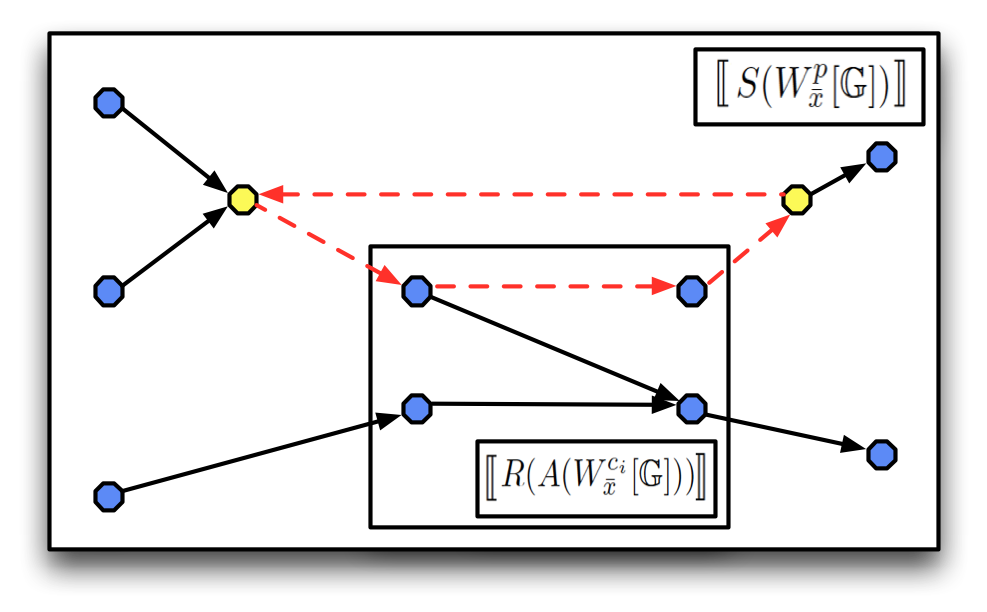
\includegraphics[width=0.7\columnwidth]{figures/abstracted_graph.png}}
    \caption{Abstract hierarchical graph model}
    \label{fig:abs_cycle}
    \end{center}	
\end{figure}

\subsection*{Algorithm Description}
\addcontentsline{toc}{subsection}{Algorithm Description}

Assume we have a function 
${\scriptstyle \mathrm{FINDALLCYCLES}}: \mathbb{G} \rightarrow \mathbf{2}^{\mathbb{G}}$
which enumerates all elementary cycles in a graph $\mathbb{G}$, 
returning sets of subgraphs.  Then Algorithm \ref{alg:hcycles} 
adapts the general algorithm
${\scriptstyle \mathrm{FINDALLCYCLES}}$ to the hierarchical graph 
structure described above.  We 
assume that $\mathbb{G}$ has a unique root design, and that we have a 
function $modified: \mathbb{D} \rightarrow boolean$ which indicates whether
a particular hierarchical component has been modified since the last run.
New components in the model are considered modified by default.

\begin{algorithm}[H]
\caption{Hierarchical cycle detection}
\label{alg:hcycles}
\begin{algorithmic}[1]
\State $cycles \gets [ ]$
\State $ifaces \gets \{ \}$
\Function{findhcycles}{ $ \llbracket W_{\bar{x}}^p [\mathbb{G}] \rrbracket$ }
   \ForAll { $W_{\bar{x}_i}^{c_i} [\mathbb{G}] \in W_{\bar{x}}^p [\mathbb{G}]$  }
      \State ${\scriptstyle \mathrm{FINDHCYCLES}}( \llbracket W_{\bar{x}_i}^{c_i} [\mathbb{G}] \rrbracket )$
   \EndFor
   \State $modified( W_{\bar{x}}^p [\mathbb{G}]) \gets (modified( W_{\bar{x}}^p [\mathbb{G}]) \vee ( \vee_{c_i} modified( W_{\bar{x}_i}^{c_i} [\mathbb{G}] ) )$
   \If { $modified( W_{\bar{x}}^p [\mathbb{G}])$ }
      \State $T \gets \llbracket S(W_{\bar{x}}^p [\mathbb{G}] \rrbracket )$
      \State $cycles \gets [ cycles; {\scriptstyle \mathrm{FINDALLCYCLES}}( T ) ]$
      \State $ifaces[p] \gets A(T)$
   \EndIf
\EndFunction
\State ${\scriptstyle \mathrm{FINDHCYCLES}}( \mathbb{G}) $
\end{algorithmic}
\end{algorithm}


\begin{itemize}
\item (Lines 1-2) We initialize a list to contain the resulting cycles, and an associative list to contain the interface data.
\item (Lines 3-6) The algorithm performs a depth-first search on the hierarchical graph, recursively visiting all of the child components ($W_{\bar{x}_i}^{c_i} [\mathbb{G}]$)  for the current (parent) component ($W_{\bar{x}}^p [\mathbb{G}]$) which is currently under evaluation.
\item (Line 7)  The modification status is propagated up the hierarchy as the algorithm progresses.  Each component which has a modified child will also be marked as modified.
\item (Lines 8-12) If the current component has been modified, we use the previously computed incremental connectivity interface for each subcomponent to check for cycles in the parent component -- the connectivity graph interface is substituted for each subcomponent.  The cycles are accumulated as the algorithm ascends to the top of the model, and a connectivity interface is created for the current component as well.
\end{itemize}

The runtime for the extended algorithm should be slightly worse than Johnson's 
algorithm in the worst case, as it must also compute the interface graphs.  
In the average case the cycle checking proceeds on graphs much smaller than
the global graph, offsetting the cost of finding paths in each subgraph.
Further, if the incremental interface edges are stored in the model following
the analysis, then scalability is enhanced when incrementally adding functions to a design.  Cycle analysis is then restricted to the size of the new components together with the stored interfaces.
